\clearpage
\newpage
\section{Overall Description}
\label{sec:general_disc}

\subsection{Scenarios}
\begin{enumerate}
    \item {\textbf{Create Tournament}}\newline
    Håkon teaches a class in introduction to programming at Middelfart Gymnasium and is teaching his class about basic programming logic.
    The students have a hard time grasping the concepts, so he decides to use CodeKataBattles to allow them to apply the theory in practice.
    He creates a tournament named “Introduction2Programming” for the class and asks all participants to create a user and subscribe to the tournament. 
    \item {\textbf{Create a Battle}}\newline
    Håkon is preparing a battle for the Introduction2Programming tournament on recursive programming. 
    He creates the required build automation scripts, test cases and description, uploads it to the battle and specifies the number of students and relevant deadlines. 
    Due budget cuts he does not have time to give personal feedback so he sets the scoring configuration to automatic. 
    \item {\textbf{Register a Team}}\newline
    Torben receives a notification from a tournament about a new Battle in a tournament he is participating in. 
He logs into CKB and reads the specifications of the new battle and sees that the registration deadline expires tomorrow. 
Groups may contain up to 4 participants so he registers a team 'TorbensTæskehold' and invites his 3 classmates.
    \item {\textbf{Participate in a Battle}}\newline
    Bertram is participating solo in a battle due to his lack of social skills. 
    The registration deadline has just ended so he receives a link for a GitHub repository titled “binary\_search”. He forks the repository and sets up the required automated workflow through GitHub Actions, allowing the platform to grade and test his solution. 
    \item {\textbf{Receive an evaluation}}\newline
    Bertram pushes a new commit to his forked repository “binary\_search” with a new solution to the battle. After a few minutes, he receives a notification that he has received a new score in this battle. To his dismay, he realizes that the assigned score is 0/100 and places him dead last in the current rankings. 
    \item {\textbf{Assign Manual Score}}\newline
    The submission deadline for the battle “binary\_tree\_inversion” has now been transgressed. 
Since Håkan has specified that scores include manual feedback, the battle now enters a consolidation phase. 
He assigns additional scores based on the code’s similarity to his own solution and updates the score for each participant. 
    \item {\textbf{Receive a Badge}}\newline
    Jørgen has just finished participating in the battle “birds\_on\_a\_line” where I placed 2nd. He receives a notification that he has placed top 3 in 5 battles in a row in the current tournament, earning him the badge “CodeNinja”. He is very pleased and calls his mother.  
\end{enumerate}

\subsection{Product perspective}

The Domain Class Diagram depicted below illustrates the structure and relationships within the CodeKataBattle system's class domain. This diagram is instrumental in understanding the interactions among the various elements of the system. Below are highlighted the most salient relationships and their constraints to facilitate comprehension of the system's domain.

\begin{itemize}
    \item \textbf{Educator and User:} The system distinguishes between two types of users: students and educators, each being a specialized type of User. Every Educator can create multiple Tournaments and Battles, representing a one-to-many relationship (\texttt{1..*}). This design choice reflects the need for Educators to manage various coding challenges and competitive events within the platform.  

    \item \textbf{Tournament:} Tournaments are each uniquely created and owned by an Educator, but an Educator can create multiple Tournaments implying a one-to-many relationship (\texttt{1..*}) regarding creation. Tournaments can encompass multiple Battles (\texttt{0..*}) and can linked to many Users who participate in them, indicating a 0-to-many relationship (\texttt{0..*}). 

    \item \textbf{Battle:} Battles, the individual challenges within Tournaments, are designed to accommodate participation by multiple Groups, with a multiplicity of zero-to-many (\texttt{0..*}). Each Battle is capable of receiving multiple Submissions from each Group.

    \item \textbf{Group:} The Group entity denotes teams of Users (students) who participate in Battles. A Group can consist of one or more Users, thus forming a many-to-many relationship (\texttt{*..*}) with the User entity. 
    
    \item \textbf{Submission:} Submissions are created by Groups and are associated with specific Battles. Each Submission is linked to one Battle, signifying a one-to-one relationship (\texttt{1..1}) in the context of evaluation. However, a Battle can have numerous Submissions linked to it, showcasing a one-to-many relationship (\texttt{1..*}).

    \item \textbf{Notification:} Notifications are triggered by system events and are sent to Users. A Notification has a \texttt{(*..1)}  relationship to Tournament, as a Notification will always be sent due to events in the tournament, battles within the tournament, submission to the battle in the tournament or badges achieved in the tournament. This implies a (\texttt{0..*}) relationship from certain classes to Notifications, as a Notification \textit{can} be triggered by a Battle, Badge or submission, but not necessarily by any of them.  A many-to-many relationship (\texttt{*..*}) exists from a Notification to a Student, indicating that each Notification can be sent to a variety of Student (e.g. Registration Deadline Has Ended) and that a Student can receive several Notifications.

    \item \textbf{Badge:} The Badge entity is connected to Users based on their achievements within the system. Multiple Badges can be awarded to a single User, and many users can achieve a badge, highlighting a many-to-many relationship (\texttt{*..*}).
\end{itemize}

\begin{figure}[htbp!]
    \centering
    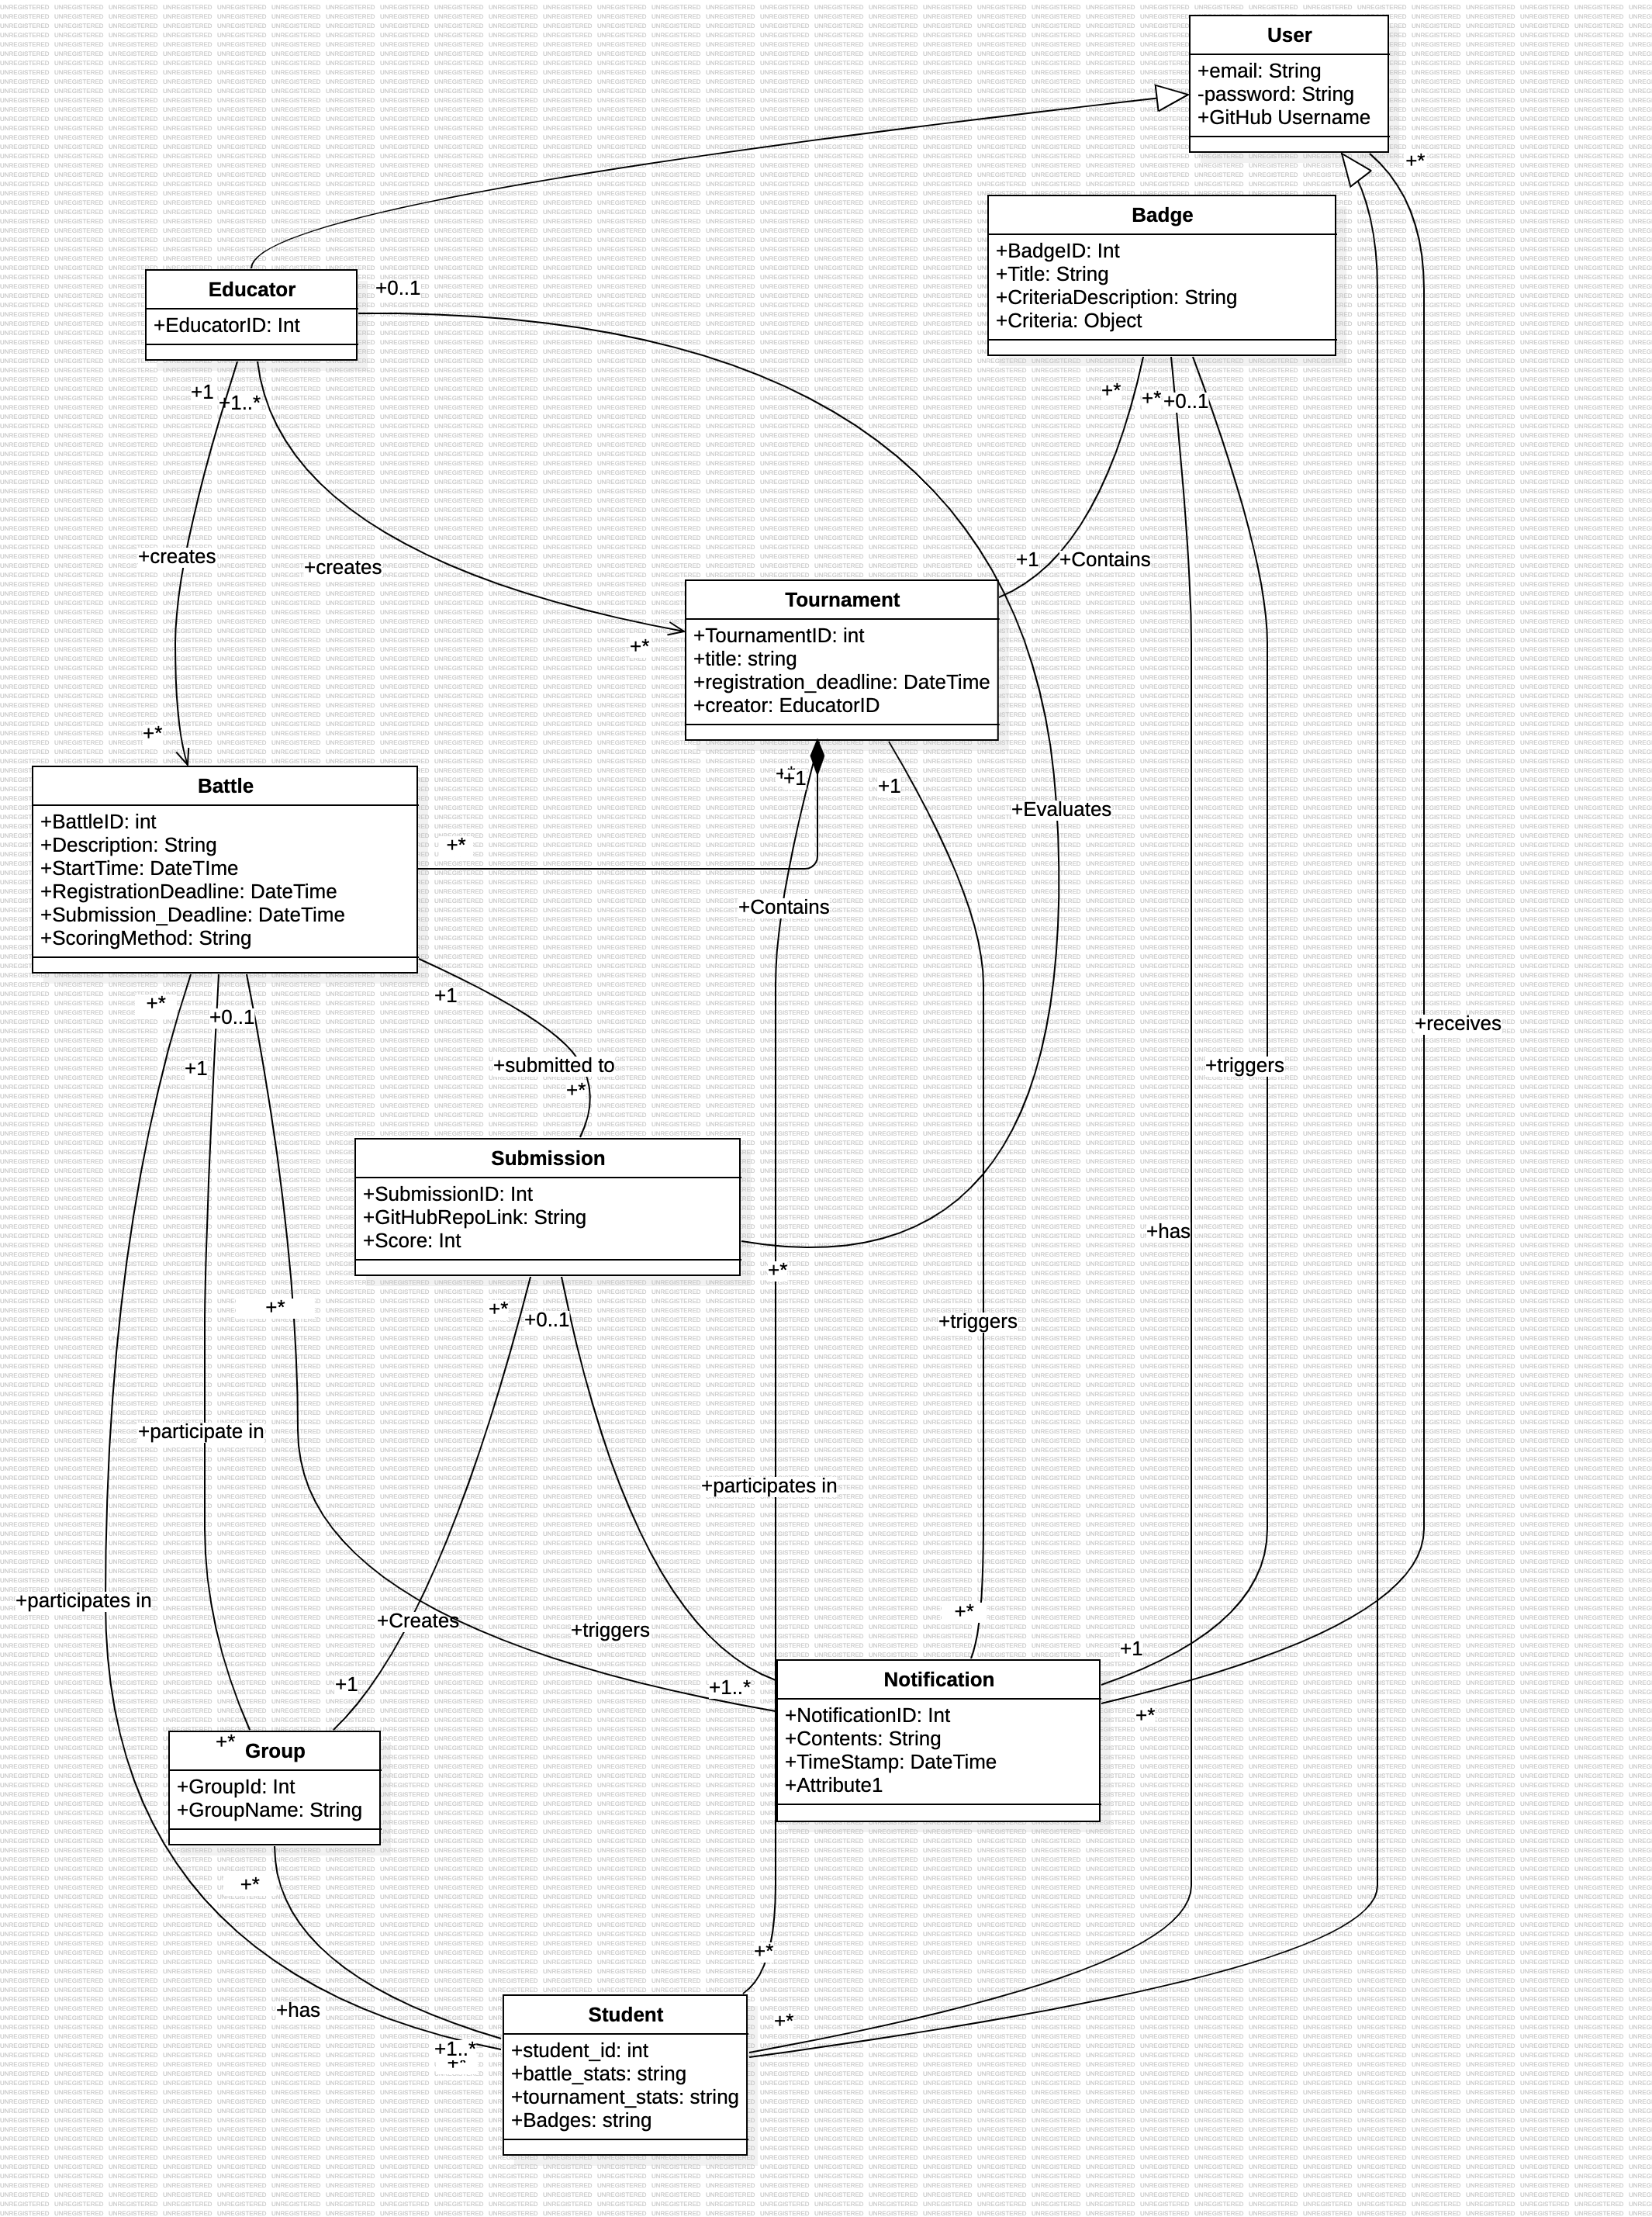
\includegraphics[width=\textwidth]{Graphics/Main.png}
    \caption{UML Domain Class Diagram}
    \label{fig:ClassDiagram}
\end{figure}


\subsection{State charts}

These two state diagrams gives an overview over the two most essential process within CodeKataBattles, namely the Battle and Tournament. 

\begin{figure}[htbp]
    \centering
    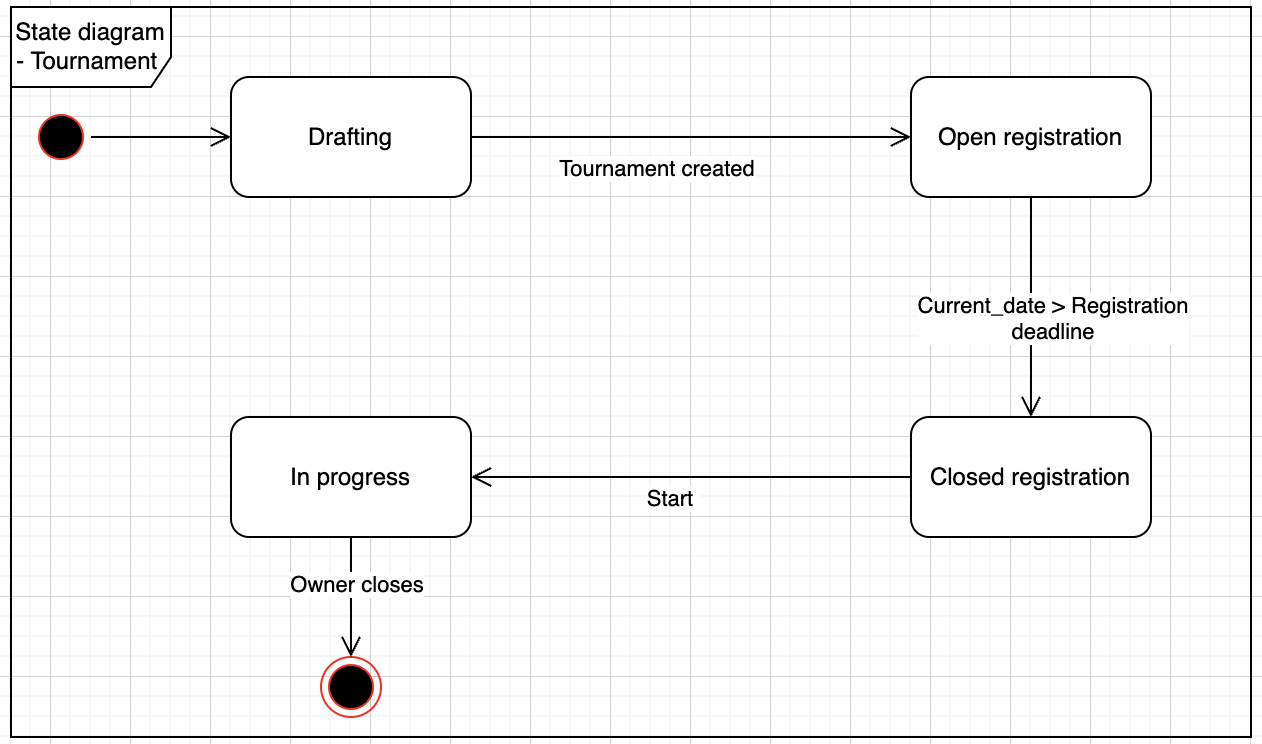
\includegraphics[width=\textwidth]{Graphics/State Diagram/Tournament.png}
    \caption{State Diagram - Tournament}
    \label{fig:TStateDiagram}
\end{figure}
Figure \ref{fig:TStateDiagram} shows the progression of a tournament in CodeKataBattles. Initiated by an educator, the "Drafting" phase involves filling in the tournament's details such as the title and registration deadline. Once established, the system transitions the tournament to "Open registration," allowing students to join until the deadline, after which it moves to "Closed registration." When the start date is surpassed, the tournament enters the "In progress" stage, which is where the battle can be had. This continues until the educator decides to end the event, bringing the tournament to its end and finalizing the standings.
\begin{figure}[htbp]
    \centering
    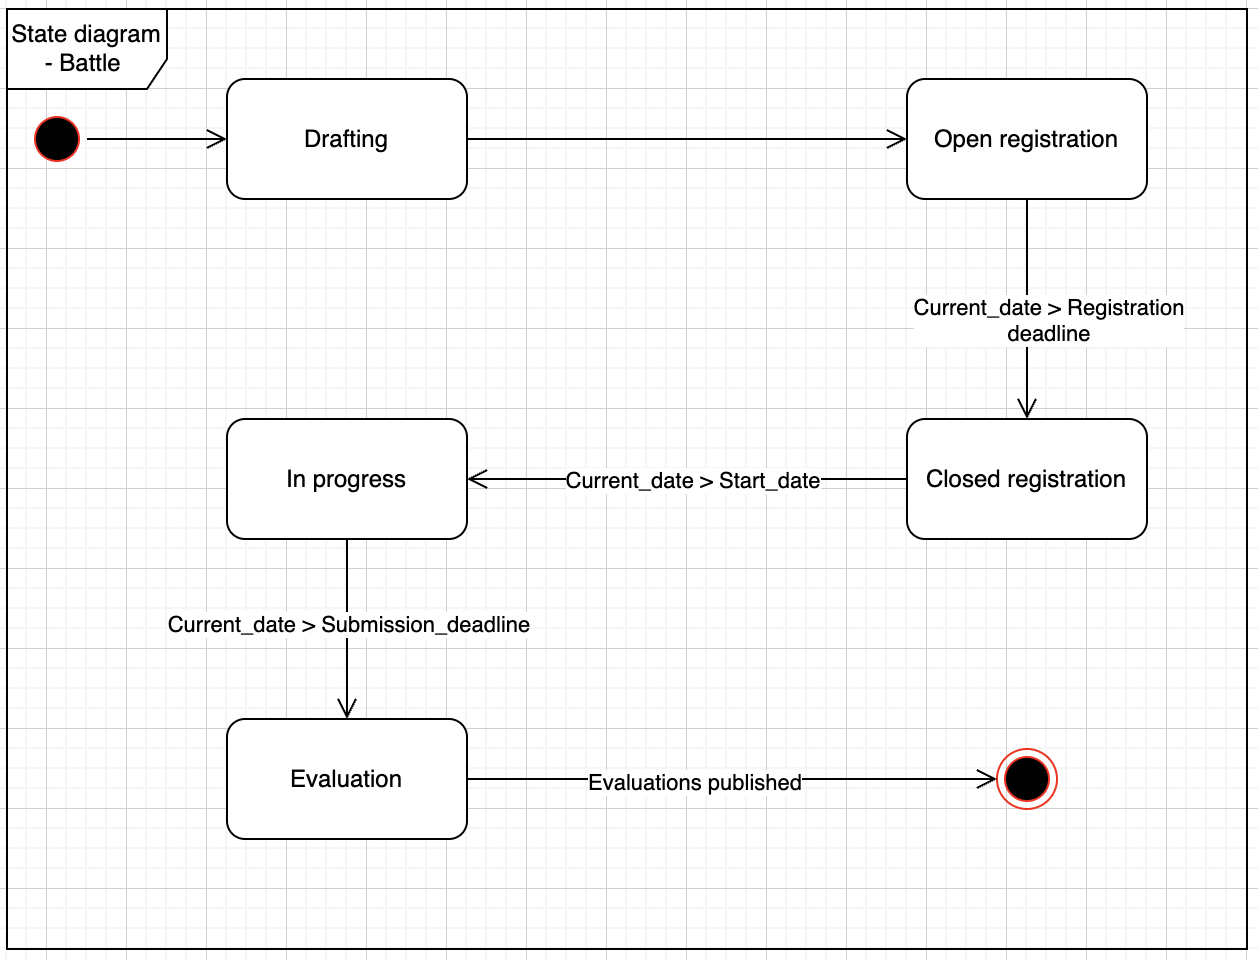
\includegraphics[width=\textwidth]{Graphics/State Diagram/Battle.png}
    \caption{State Diagram - Battle}
    \label{fig:BStateDiagram}
\end{figure}

Figure \ref{fig:BStateDiagram} displays the lifecycle of a battle within CodeKataBattles. A battle initial state the "Drafting" starts when an educator decides to create a battle within a tournament. Here the educator details the deadlines, the title, the description, and the automation scripts containing the test cases. Once that is done, and the battle's details are validated by the system, the battle is created and precedes to be open for registration. Here students within the tournament can in teams of 1 or more join the battle, however, once the registration deadline is passed the battle is closed for registrations. This waiting state is over when the start date of the battle is surpassed, commencing the "in progress" stage of the battle. Here students can submit as many solutions for the problem and get feedback. The stage ends when the submission deadline is finished. Now all the team's best solutions are put into the final ranking, and every participant in the battle is notified. Hereafter the Battle has ended.  
\subsection{Product functions}

The following section will have a detailed description of the CodeKataBattles functions. 


\begin{enumerate}
    \item {\textbf{Sign-Up \& Log In}}\newline
    This functionality should enable the user to register as a user on the platform. Each user has to specify their email and their GitHub username. We will use the email as their username, and let them specify their passwords under standard security requirements. For the user to finalize their registration, and verification email is sent to the given email with a link for the user to confirm their access to the email. After the initial sign-up process is finished, the user can log on to the platform via their specified email and password. 
    \item {\textbf{Create battle}}\newline
    Available to every educator is the ability to create a battle under a given tournament, where the educator has the required permissions. The educator then needs to specify a number of elements to finalize the creation of the battle. One element concerns the technical documents making up the code kata. Here the educator is required to specify a description of the battle, test cases specifying how a satisfactory solution should behave, and lastly include the automation scripts. Thereafter the educator has to make the formal configuration of the code kata, which entails setting the minimum and maximum size of the groups and setting the registration and final submission deadline. The last element to specify is the configuration of the scoring methodology for the battle. Here the educator can enable manual scoring or automate the process in a weighted manner to their liking. 
    \item {\textbf{Join battle}}\newline
    Students can see the tournaments open for registration, and the open battles, in tournaments they already have joined. When selecting to join a battle, the user is prompted to create a group. The group can consist of the sole creator of the group, or the student can invite as many additional students as the battle allows. The other students need to already be registered for the tournament to be able to be invited. Each group needs a name unique to the battle participants. 
    \item {\textbf{Create tournament}}\newline
    Only an educator can create a tournament. A tournament requires a title, registration deadline, and specification of badges for the tournament. Each badge needs a title, and a set of rules enabling the automation of giving out the badge to participants that fulfill the requirements for the badge. Beyond the registration deadline putting a threshold of when students can join the battle, the deadline also constrains battle deadlines in the tournaments to be after the battle. To enable other educators to create battles within the tournament, the original creator of the tournament has to add the educator by username to a list of educators with permission. 
    \item {\textbf{Receive Notifications from battles}}\newline
    When a student or group has joined a battle they are placed on a notification list that enables them to receive notifications in several scenarios:
    \begin{enumerate}
        \item When the registration deadline is transgressed users receive a link to the GitHub repository containing code descriptions, build automation scripts, and other relevant files. 
        \item When a submission has been evaluated the user receives a notification containing indexes of the tests that the program has passed as well as the score for the solution.
        \item When the submission deadline is transgressed the user receives a notification with the final score and rank in the battle.
    \end{enumerate}
    \item {\textbf{Receive Notifications from Tournaments}}\newline
    If a user is subscribed to a tournament the user is placed on a notification list so they can be notified in certain situations. The user is notified when a battle is created under a tournament. The user is notified of their tournament rank \& score when the tournament is ended by a permitted educator. The user is notified if they qualify for any badges specified in the tournament. 
    \item {\textbf{See tournament information}}\newline
    In order to keep up with their performance and upcoming battles, users can inspect Tournament information. This includes seeing previous, future, and ongoing battles of the tournaments along with relevant summary statistics, such as average score and number of participants. Additionally, the user can see their current rank and score on the tournament leaderboard. Users can also inspect if they have received any badges in the tournament. 
    \item {\textbf{See battle information}}\newline
    This functionality allows users to keep up with the battles they are involved in. This includes seeing the attempts made by the user or group along with the number of tests passed by each attempt. The battle leaderboard reveals the rank and score of the user or group in the current battle. The information on remaining time until the submission deadline and the number of participants is also visible.

    \item {\textbf{Display Student Profile}}\newline
    This functionality allows students and educators to view student's battle and tournament involvement. This includes rankings, badges and achievements. 
\end{enumerate}

\subsection{User characteristics}
The CodeKataBattles system is primarily interacted with by two categories of users: Students and Educators.

\subsubsection{Student}
In the context of CodeKataBattles, a student is a type of user registered on the CodeKataBattle platform solely for participating in code kata battles and tournaments. They cannot create battles or tournaments. They have a device with an internet browser and internet connection so they can access the web application. 

\subsubsection{Educator}
In the context of CodeKataBattles, an educator is a type of user registered on the CodeKataBattle platform for creating and hosting tournaments in code kata battles and tournaments. They can also score submissions in battles where manual evaluation is enabled and she/he is owner of the tournament. They can also close down tournaments at will.
They have a device with an internet browser and internet connection so they can access the web application. 


\subsection{Assumptions, dependencies and constraints}

\subsubsection{Regulatory Policies}
The CodeKataBattle platform will ask for user personal information like email address linked with a GitHub user. Email addresses and Github user information won’t be used for commercial purposes. Personal information will be processed in compliance with the GDPR.


\subsubsection{Domain Assumptions}
\label{sec:domain_assumptions}

This section outlines the assumptions that are considered as given within the operational domain of the CodeKataBattle system. These are conditions that the system presumes to be true and are necessary for the correct operation and use of the platform.

\begin{enumerate}
    \item \textbf{[D1]} Users must have a stable internet connection to access and interact with the CodeKataBattle platform.
    \item \textbf{[D2]} Users' computing devices must be capable of running the necessary software development tools for coding battles.
    \item \textbf{[D3]} GitHub services are available and reliable as the platform depends on GitHub for repository hosting and Actions for automated workflows.
    \item \textbf{[D4]} Educators and students must have a basic understanding of how to use version control systems, particularly GitHub.
    \item \textbf{[D5]} Automated testing scripts provided in code katas are correct and capable of accurately evaluating the students' code submissions.
    \item \textbf{[D6]} Users must allow notification services to receive timely updates from the CodeKataBattle platform.
    \item \textbf{[D7]} The static analysis tools integrated with the platform for code quality assessment are functioning and accessible.
    \item \textbf{[D8]} Students' submissions through GitHub are timestamped accurately to ensure fair evaluation of timeliness.
    \item \textbf{[D9]} Educators inputting the battle information, including test cases and scoring configurations, must ensure their accuracy and clarity.
    \item \textbf{[D10]} The computing environment used by students for development is compatible with the code kata requirements and specifications.
    \item \textbf{[D11]} The system's timekeeping is synchronized with an accurate time source to ensure deadline enforcement.
    \item \textbf{[D12]} Educators are responsible for defining clear and measurable objectives for battles and tournaments.
    \item \textbf{[D13]} Students are expected to follow the test-first approach as specified in the battle requirements, creating tests before implementation.
    \item \textbf{[D14]} Scores and feedback are assumed to be constructive and used for educational purposes, not as punitive measures.
    \item \textbf{[D15]} The platform assumes all users act in good faith, not attempting to game the system or manipulate scores through unfair means.
\end{enumerate}


\newpage